\documentclass{article}
\usepackage[table]{xcolor}
\usepackage{titlepic}
\usepackage{hyperref}
\usepackage{amsmath}
\usepackage{enumitem}% http://ctan.org/pkg/enumerate
\usepackage{rotating} 
\usepackage{float}
\usepackage{multirow}
\usepackage[margin=0.5in]{geometry}
\usepackage{titling}
\usepackage{capt-of}
\usepackage{siunitx}
%\usepackage{arydshln}
\usepackage{longtable}
\usepackage{xcolor}
\usepackage{colortbl}
%\usepackage[justification=centering]{caption}
%\usepackage{caption}
\sisetup{group-separator = {,}, group-minimum-digits = 4}
\definecolor{CSONavy}{HTML}{405381}
\hypersetup{
    colorlinks,
    linkcolor={black!50!black},
    citecolor={blue!50!black},
    urlcolor={blue!80!black}
}
\urlstyle{same}
%\nocite{*}
%\setlength{\droptitle}{-4.5em}

%\titlepic{\includegraphics{../figures/CSO_Logo.png}}
\title{CHN Health Profile - a (IHA: One ;  Health Region: HSE Dublin and South East) }
%\date{\vspHRe{-5ex}}
\date{Census 2022}
\author{CSO, Ireland  (\url{http://www.cso.ie)}}

\newcolumntype{T}{>{\raggedleft\arraybackslash}m{1.7cm}}
\newcolumntype{O}{>{\centering\arraybackslash}m{3.4cm}}
\newcolumntype{M}{>{\raggedleft\arraybackslash}m{3cm}}
\newcolumntype{A}{>{\raggedright\arraybackslash}m{9.5cm}}
\newcolumntype{S}{>{\raggedleft\arraybackslash}m{1.4cm}}
\newcolumntype{K}{>{\raggedright\arraybackslash}m{7.5cm}}

\usepackage{Sweave}
\begin{document}
\Sconcordance{concordance:1-a-ac-hse-dublin-and-south-east.tex:HealthProfileTemplate.Rnw:1 44 1 1 0 845 1}

%\includegraphics{../figures/CSO_Logo.png}
%\begin{minipage}{\linewidth}

\begin{figure}
	\centering
\includegraphics[width =75mm]{../figures/CSO_Logo.png}
\end{figure}

				 
		   
						  
														  
																																													
												 
			 
\maketitle
					
													   
				 
						 
																																																																											   
				 
				  
  \pagebreak
    	    \tableofcontents
%\end{minipage}

\pagebreak


\section{Key Points}

\begin{itemize}

\item The \textbf{Age Dependency Ratio} of this Electoral Division (ED) is  \textbf{55.9}. This compares to 53.2 nationally. The Age Dependency Ratio is the amount of people outside of working age (0-14 and 65+) per 100 people of working age (15-64). 

\item a has a total of \textbf{\num{764}} \textbf{persons} and  \textbf{\num{213}} \textbf{families} living in private households.

\item There are a total of \textbf{151 persons aged 0-14} in this ED and \textbf{123 persons aged over 65.} 

\item There are a total of \textbf{\num{168}} persons \textbf{living with a disability} in this ED, representing \textbf{22.0 percent} of the population. This compares with  21.5 percent nationally

\item \textbf{\num{14}} people in this ED have \textbf{bad or very bad general health}. This represents \textbf{1.8 percent} of the population. 1.7 percent of the population have bad or very bad general health nationally. 

\item There are a total of \textbf{\num{70} carers} in this ED, representing \textbf{9.2 percent} of the population. This compares with 5.8 percent of the population that are carers nationally. 

\item \textbf{8.2 percent} of this ED \textbf{smoke tobacco products}. 13.1 percent of people nationally smoke tobacco products

\item There are \textbf{\num{6} short term unemployed} and \textbf{\num{12} long term unemployed} people in this ED. These represent 1.0 and 2.0 percent of the population respectively.

\item  \textbf{2.4 percent} of the population of a are \textbf{unskilled}. 3.1 percent of people in the state are unskilled.

\item \textbf{23.5 percent} of those aged 15+ in this ED have a \textbf{highest level of education of lower secondary or lower}. This compares with 23 percent nationally. 

\item \textbf{14.4 percent} of families with children in this ED have \textbf{lone parents}. This stands at 24.8 nationally.

\item \textbf{5.3 percent} of this ED were \textbf{born outside Ireland} (20 percent nationally).

\item \textbf{Households rented from a Local Authority} comprise \textbf{0.8 percent} of households in this ED.This stands at 8.3 percent nationally

\end{itemize}

\pagebreak

\section{Population} 
\label{sect:Pop}

\begin{figure}[h]
	\centering
	\includegraphics[width = 100mm]{../figures/PyramidPlot.pdf}
	\caption{Persons by Age Group and Gender for a; Health Region and State; Census 2022.}
	\label{fig:2ae19629-1a6a-13a3-e055-000000000001}
	\end{figure}

\begin{table}[!h]
\centering
\begin{tabular}{lSSSSSSSSSS}
  \hline
 \textbf{Age} & \multicolumn{2}{c}{\textbf{Females}} & \multicolumn{2}{c}{\textbf{Males }} & \multicolumn{5}{c}{\textbf{Both Sexes}}  \\ 
\cline{6-9}\\
 & \emph{\textbf{Persons}} & \emph{\textbf{\%}} & \emph{\textbf{Persons}} & \emph{\textbf{\%}} & \emph{\textbf{Persons}} & \emph{\textbf{\% (ED)}} & \emph{\textbf{\% (IHA)}}& \emph{\textbf{\% (HR)}}& \emph{\textbf{\% (State)}}\\
  \hline
  0-14   & 74 &  19.7 & 77 & 19.8 & 151 &19.8 & 22.4& 19.1 & 19.7 \\
  15-64  & 243 & 64.6 & 247 & 63.7 & 490&64.1& 65.9 & 64.4 &65.3\\
  65+ & 59 & 15.7 & 64 & 16.5 &123 &16.1 & 11.7& 16.4 & 15.1 \\
 \hline
  Age 0-4  & 18& 4.8& 18 & 4.6& 36 & 4.7 & 4.5& 5.5& 5.7 \\
  
  Age 5-9  & 31& 8.2& 21 & 5.4& 52 & 6.8 & 6.9& 6.5& 6.7 \\

  Age 10-14  & 25& 6.6& 38 & 9.8& 63 & 8.2 & 11.0& 7.1& 7.3 \\

  Age 15-19  & 30& 8.0& 28 & 7.2& 58 & 7.6 & 7.9& 6.4& 6.6 \\

  Age 20-24  & 15& 4.0& 22 & 5.7& 37 & 4.8 & 4.8& 5.8& 6.0 \\

  Age 25-29  & 13& 3.5& 13 & 3.4& 26 & 3.4& 3.8 & 5.6& 5.7 \\

  Age 30-34  & 12& 3.2& 22 & 5.7& 34 & 4.5 & 6.4& 6.2& 6.5 \\

  Age 35-39  & 26& 6.9& 23 & 5.9& 49 & 6.4 & 4.5& 7.0& 7.4 \\

  Age 40-44  & 33& 8.8& 30 & 7.7& 63 & 8.2 & 9.5& 7.8& 8.0 \\
  
    Age 45-49  & 34& 9.0& 32 & 8.2& 66 & 8.6 & 9.1& 7.2& 7.3 \\
  
    Age 50-54  & 21& 5.6& 30 & 7.7& 51 & 6.7 & 6.9& 6.7& 6.6 \\
  
    Age 55-59  & 26& 6.9& 23 & 5.9& 49 & 6.4 & 6.2& 6.3& 6.0 \\
  
    Age 60-64  & 33& 8.8& 24 & 6.2& 57 & 7.5 & 6.7& 5.6& 5.3 \\
  
    Age 65-69  & 16& 4.3& 19 & 4.9& 35 & 4.6 & 5.0& 4.9& 4.6 \\
  
    Age 70-74  & 15& 4.0& 16 & 4.1& 31 & 4.1 & 2.1& 4.2& 3.9 \\
  
    Age 75-79  & 14& 3.7& 18 & 4.6& 32 & 4.2 & 2.1& 3.3& 3.0 \\
  
    Age 80-84  & 6& 1.6& 6 & 1.5& 12 & 1.6 & 1.4& 2.2& 1.9\\
  
    Age 85 and over  & 8& 2.1& 5 & 1.3& 13 & 1.7 && 1.0 1.9& 1.6 \\
  
    All Ages  & 376& 100.0& 388 & 100.0& 764 & 100.0 & 100.0& 100.0& 100.0 \\
      \hline 
    \multicolumn{4}{l}{\href{https://data.cso.ie/table/SAP2022T1T1AED}{https://data.cso.ie/table/SAP2022T1T1AED}} & & &
\end{tabular}
\caption{Population Breakdown by Age and Sex for a; Census 2022. Percentage breakdowns for Health Region (HR) and State are provided for comparison purposes.}
\end{table}

\pagebreak

\section{Disability}\label{sect:Disability}
\begin{figure}[h]
	\centering
	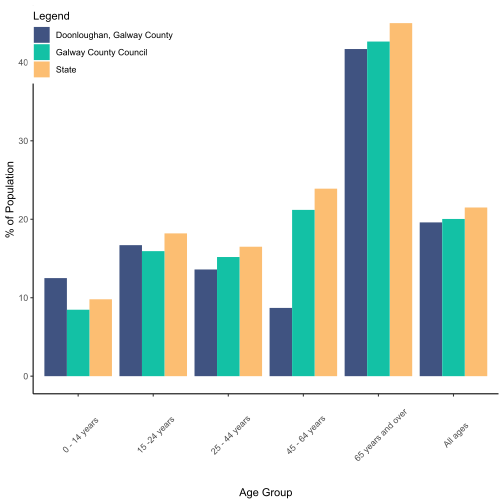
\includegraphics[width = 130mm]{../figures/DisED.pdf}
	\caption{Percentage of Population with any Disability by Age Group for a; Health Region and State; Census 2022.}
	\label{fig:2ae19629-1a6a-13a3-e055-000000000001}
	\end{figure}


\begin{table}[!h]
\centering
\begin{tabular}{lTTTTTT}
  \hline
 & \multicolumn{3}{c}{\textbf{a}} & \textbf{IHA}& \textbf{HSE Dublin and South East} & \textbf{State}\\ 
 \cline{2-4} \\
  \textbf{Age Group} & \textbf{Population} & \multicolumn{4}{c}{\textbf{With any Disability}} \\
 \cline{3-6}\\
& \emph{\textbf{Persons}} & \emph{\textbf{Persons}} & \emph{\textbf{\%}} & \emph{\textbf{\%}} & \emph{\textbf{\%}}& \emph{\textbf{\%}}\\
  \hline
Males & \num{388} & \num{78}  & 20.1  & 16.6666666666667 & 21.8 & 20.9\\
Females & \num{376} & \num{90}  & 23.9  & 21.5& 23.1& 22.2\\
Both Sexes & \num{764} & \num{168}  & 22.0  & 21.5& 23.1& 21.5 \\
   \hline
       \multicolumn{5}{l}{\href{https://data.cso.ie/table/F4004}{https://data.cso.ie/table/F4004}} & 
\end{tabular}
\caption{Population with any Disability by Age Group for a; Census 2022. Percentage breakdowns for Health Region and State are provided for comparison purposes.}
\end{table}

\pagebreak

\section{General Health}\label{sect:GenHealth}

\begin{figure}[h]
	\centering
	\includegraphics[width = 150mm]{../figures/GenED.pdf}
	\caption{Population Breakdown (\%) by General Health for a; Health Region and State;  Census 2022.}
	\label{fig:2ae19629-1a6a-13a3-e055-000000000001}
	\end{figure}

\begin{table}[!h]
\centering
\begin{tabular}{lTTTTT}
  \hline
\textbf{General Health} & \multicolumn{2}{c}{\textbf{a}} & \textbf{IHA}& \textbf{HSE Dublin and South East} & \textbf{State}\\ 
 \cline{2-3} \\
 & \emph{\textbf{Persons}} & \emph{\textbf{\%}} & \emph{\textbf{\%}} & \emph{\textbf{\%}}& \emph{\textbf{\%}} \\
  \hline
Very Good& \num{442} &57.9
&58.9
&55.4 &53.2 \\
Good& \num{230} &30.1 &29.8 &29.3 &29.7\\
Fair& \num{60} &7.9 &5.7 &8.5 &8.6\\
Bad& \num{11} &1.4 &1.2 &1.4 &1.4\\
Very Bad& \num{3} &0.4 &0.5 &0.3 &0.3\\
Not Stated& \num{18} &2.4 &3.8 &5.2 &6.7\\
Total& \num{764} &100.0 &100.0 &100.0 &100.0\\
   \hline
       \multicolumn{5}{l}{\href{https://data.cso.ie/table/SAP2022T12T3ED}{https://data.cso.ie/table/SAP2022T12T3ED}} & 
\end{tabular}
\caption{Population by General Health for a; Census 2022. Percentage breakdowns for Health Region and State are also provided for comparison purposes.}
\end{table}
\pagebreak

\section{Carers}\label{sect:Carers}
\begin{figure}[H]
	\centering
	\includegraphics[width = 150mm]{../figures/CareED.pdf}
	\caption{Carers as a Percentage of the Population of Males/Females/Both Sexes for a; Health Region and State; Census 2022.}
	\label{fig:2ae19629-1a6a-13a3-e055-000000000001}
	\end{figure}
	
	
\begin{table}[!h]	
\centering
	\begin{tabular}{lTTTTTT}
  \hline
 & \multicolumn{3}{c}{\textbf{a}} & \textbf{IHA}& \textbf{HSE Dublin and South East} & \textbf{State}\\ 
 \cline{2-4} \\
  \textbf{Age Group} & \textbf{Population} & \multicolumn{5}{c}{\textbf{Carers}} \\
 \cline{3-6}\\
& \emph{\textbf{Persons}} & \emph{\textbf{Persons}} & \emph{\textbf{\%}} & \emph{\textbf{\%}}& \emph{\textbf{\%}} & \emph{\textbf{\%}}\\
  \hline
Males & \num{388} & \num{31}  & 8.0  & 10.0  & 4.6 & 2.3 \\
Females & \num{376} & \num{39}  & 10.4  & 8.6 & 7.2 & 3.5 \\
Both Sexes & \num{764} & \num{70}  & 9.2  & 9.3& 6.0 & 5.8 \\
     \hline
       \multicolumn{3}{l}{\href{https://data.cso.ie/table/SAP2022T12T2ED}{https://data.cso.ie/table/SAP2022T12T2ED}} 
\end{tabular}

\caption{Carers by Sex for a; Census 2022. Percentage Breakdowns for Health Region and State are also provided for comparison purposes.}
\end{table} 

\pagebreak

\section{Volunteers}\label{sect:Volunteers}
\begin{figure}[H]
	\centering
	\includegraphics[width = 150mm]{../figures/VolunteerED.pdf}
	\caption{Volunteers as a Percentage of the Population for a; Health Region and State; Census 2022.}
	\label{fig:2ae19629-1a6a-13a3-e055-000000000001}
	\end{figure}
	
	
\begin{table}[!h]	
\centering
	\begin{tabular}{lTTTTTT}
  \hline
 & \multicolumn{3}{c}{\textbf{a}} & \textbf{IHA}& \textbf{HSE Dublin and South East} & \textbf{State}\\ 
 \cline{2-4} \\
  & \textbf{Population} & \multicolumn{5}{c}{\textbf{Volunteers}} \\
 \cline{3-6}\\
& \emph{\textbf{Persons}} & \emph{\textbf{Persons}} & \emph{\textbf{\%}} & \emph{\textbf{\%}}& \emph{\textbf{\%}} & \emph{\textbf{\%}}\\
  \hline
& 764 & 123  & 16.1  & 13.8   & 14.2 & 13.8 \\

     \hline
       \multicolumn{3}{l}{\href{https://data.cso.ie/table/SAP2022T7T1ED}} 
\end{tabular}

\caption{Volunteers for a; Census 2022. Percentage Breakdowns for Health Region and State are also provided for comparison purposes.}
\end{table} 

\pagebreak

\section{Smoking}\label{sect:Smoking}
\begin{figure}[H]
	\centering
	\includegraphics[width = 120mm]{../figures/SmokingED.pdf}
	\caption{Percentage of the Population who Smoke tobacco Products (Daily and Occasionally) for a; Health Region and State; Census 2022.}
	\label{fig:2ae19629-1a6a-13a3-e055-000000000001}
	\end{figure}
	
	
\begin{table}[!h]	
\centering
	\begin{tabular}{lTTTTTT}
  \hline
  \textbf{Smoking Status} & \multicolumn{2}{c}{\textbf{a}} & \textbf{IHA}& \textbf{HSE Dublin and South East} & \textbf{State}\\ 
 \cline{2-3} \\
 & \emph{\textbf{Persons}} & \emph{\textbf{\%}} & \emph{\textbf{\%}} & \emph{\textbf{\%}} & \emph{\textbf{\%}} \\
  \hline
Smoke tobacco Products (Daily and Occasionally)& \num{63} &8.2 &7.9&12.8 &13.1 \\
Don't Smoke tobacco Products (Never and have given up)& \num{679} &88.9 &87.6&81.3 &79.4 \\
Smoking Status Not Stated& \num{22} &2.9 &4.5&5.8 &7.5 \\
All Persons & 764 & 100.0 & 100.0  & 100.0 \\
     \hline
      \multicolumn{3}{l}{\href{https://data.cso.ie/table/SAP2022T12T4ED}{https://data.cso.ie/table/SAP2022T12T4ED}} 
\end{tabular}

\caption{Smoking Status of a; Census 2022. Percentage breakdowns for Health Region and State are also provided for comparison purposes.}
\end{table} 
    
  
\pagebreak
\section{Principal Economic Status}\label{sect:PES}
\begin{figure}[H]
	\centering
	\includegraphics[width = 140mm]{../figures/PESED.pdf}
	\caption{Percentage of Population Aged 15+ by Principal Economic Status for a, Health Region and State; Census 2022.}
	\label{fig:vbnv}
	\end{figure}

\begin{table}[h]	
\centering
		\begin{tabular}{lTTTTTT}
  \hline
  \textbf{Principal Economic Status} & \multicolumn{2}{c}{\textbf{a}}& \textbf{IHA} & \textbf{HSE Dublin a...} & \textbf{State}\\ 
 \cline{2-3} \\
 & \emph{\textbf{Persons}} & \emph{\textbf{\%}} & \emph{\textbf{\%}} & \emph{\textbf{\%}} & \emph{\textbf{\%}} \\
  \hline
At Work & \num{358} &58.4
&64.9
&55.1 &56.1 \\
Looking for first regular job & \num{1} &0.2 &0.0&0.8 &0.8 \\
Short term unemployed & \num{6} &1.0 &0.0&1.6 &1.7 \\
Long term unemployed & \num{12} &2.0 &1.5&2.5 &2.6 \\
Student & \num{69} &11.3
&12.0&11.0 &11.1 \\
 Looking after home/family & \num{37} &6.0 &6.2&6.9 &6.6 \\
Retired & \num{106} &17.3 &11.7 &17.2 &15.9 \\
Unable to work due to permanent sickness or disability & \num{22} &3.6 &3.7&4.4 &4.6 \\
Other & \num{2} &0.3 &0.0 &0.6 &0.7 \\
Total & \num{613} &100.0 &100.0 &100.0 &100.0 \\
\hline
       \multicolumn{5}{l}{\href{https://data.cso.ie/table/SAP2022T8T1ED}{https://data.cso.ie/table/SAP2022T8T1ED}} &
\end{tabular}

\caption{Population aged 15+ by Principal Economic Status for a; Census 2022. Percentage breakdowns for Health Region and State are also provided for comparison purposes.}
\end{table} 

\pagebreak

\section{Social Class}\label{sect:SC}
\begin{figure}[H]
	\centering
	\includegraphics[width = 140mm]{../figures/SocialClassED.pdf}
	\caption{Percentage of Population Aged 15+ by Social Class for a, Health Region and State; Census 2022.}
	\label{fig:vbnv}
	\end{figure}

\begin{table}[h]	
\centering
		\begin{tabular}{lTTTTTT}
  \hline
  \textbf{Social Class} & \multicolumn{2}{c}{\textbf{a}}  & \textbf{IHA} & \textbf{HSE Dublin and South East} & \textbf{State}\\ 
 \cline{2-3} \\
 & \emph{\textbf{Persons}} & \emph{\textbf{\%}} & \emph{\textbf{\%}} & \emph{\textbf{\%}} & \emph{\textbf{\%}} \\
  \hline
Professional workers & \num{75} & 9.8 & 11.0& 11.1& 9.3\\
Managerial and technical & \num{287} & 37.6 & 38.4& 33.2& 30.7\\
Non-manual & \num{122} & 16.0 & 12.4&& 15.7& 16.2\\
Skilled manual & \num{124} & 16.2 & 16.9& 11.8& 12.9\\
Semi-skilled & \num{76} & 9.9 & 9.5& 10.6& 11.2\\
Unskilled & \num{18} & 2.4 & 3.1& 2.8& 3.1\\
All others gainfully occupied and unknown & \num{62} & 8.1 & 8.6& 14.9& 16.6\\
Total & \num{764} & 100.0 & 100.0& 100.0& 100.0\\
\hline
       \multicolumn{5}{l}{\href{https://data.cso.ie/table/SAP2022T9T1ED}{https://data.cso.ie/table/SAP2022T9T1ED}} &
\end{tabular}

\caption{Population aged 15+ by Social Class for a; Census 2022. Percentage breakdowns for Health Region and State are also provided for comparison purposes.}
\end{table} 
\pagebreak
\section{Education}\label{sect:Edu}
\begin{figure}[H]
	\centering
	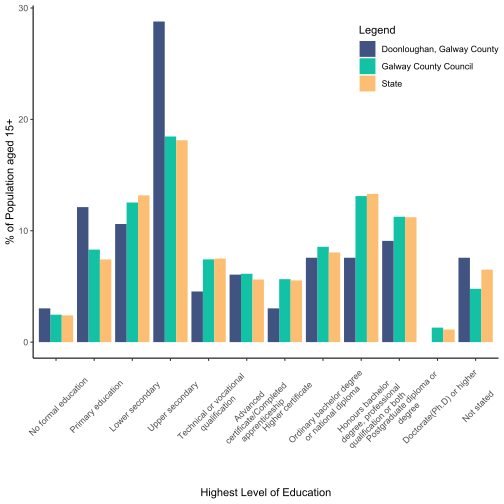
\includegraphics[width = 120mm]{../figures/EduED.pdf}
	\caption{Percentage of Population Aged 15+ by Highest Level of Education Completed for a; Health Region and State; Census 2022.}
	\label{fig:vbnv}
	\end{figure}
\begin{table}[h]	
\centering
	\begin{tabular}{lTTTTT}
  \hline
  \textbf{Highest Level of Education Completed} & \multicolumn{2}{c}{\textbf{a}} & \textbf{IHA}& \textbf{HSE Dublin and South East} & \textbf{State}\\ 
 \cline{2-3} \\
 & \emph{\textbf{Persons}} & \emph{\textbf{\%}} & \emph{\textbf{\%}} & \emph{\textbf{\%}} \\
  \hline
No formal education & \num{4} &0.8 &1.1&2.1 &2.4 \\
Primary education & \num{45} &8.6 &6.1 &6.7 &7.4 \\
Lower secondary & \num{74} &14.1 &14.1&12.9 &13.2 \\
Upper secondary & \num{76} &14.5 &13.4 &17.4 &18.1 \\
Technical or vocational qualification & \num{40} &7.6 &9.7&7.2 &7.5 \\
Advanced certificate/Completed apprenticeship & \num{46} &8.8 &8.7&5.5 &5.6 \\
Higher certificate & \num{39} &7.4 &6.1&5.5 &5.5 \\
Ordinary bachelor degree or national diploma & \num{40} &7.6 &6.9&8.2 &8.1 \\
Honours bachelor degree, professional qualification or both & \num{85} &16.2 &18.4&14.6 &13.3 \\
Postgraduate diploma or degree & \num{59} &11.3 &10.5&13.3 &11.2 \\
Doctorate(Ph.D) or higher & \num{3} &0.6 &0.4&1.4 &1.1 \\
Not stated & \num{13} &2.5 &4.7 &5.3 &6.5 \\
Total & \num{524} &100.0 &100.0 &100.0 &100.0 \\
   \hline
       \multicolumn{5}{l}{\href{https://data.cso.ie/table/SAP2022T10T4ED}{https://data.cso.ie/table/SAP2022T10T4ED}} &
\end{tabular}

\caption{Population aged 15+ by Highest Level of Education Completed for a; Census 2022. Percentage breakdowns for Health Region and State are also provided for comparison purposes.}
\end{table} 
\pagebreak    
    
\section{Families}\label{sect:Fam}
\begin{figure}[H]
	\centering
	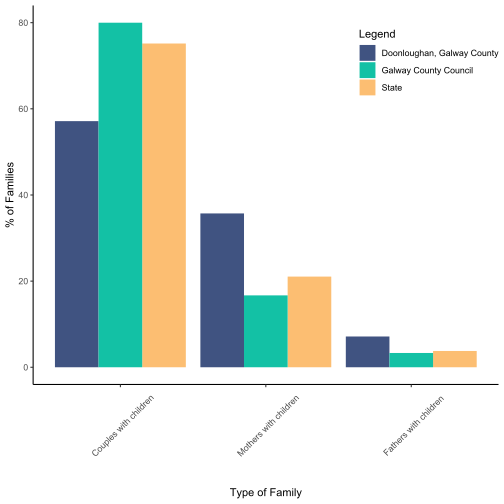
\includegraphics[width = 150mm]{../figures/FamED.pdf}
	\caption{Percentage of Families with Children by Family Type for a; Health Region and State; Census 2022.}
	\label{fig:vbnv}
	\end{figure}
	
	
\begin{table}[h]	
\centering
\begin{tabular}{lTTTTT}
  \hline
  \textbf{Type of Family} & \multicolumn{2}{c}{\textbf{a}} & \textbf{IHA}& \textbf{HSE Dublin and South East} & \textbf{State}\\ 
 \cline{2-3} \\
 & \emph{\textbf{Families}} & \emph{\textbf{\%}} & \emph{\textbf{\%}} & \emph{\textbf{\%}}& \emph{\textbf{\%}}  \\
  \hline
Couples with Children & \num{131} &85.6 &87.1 &75.2 &75.2 \\
Mothers with Children & \num{17} &11.1 &9.4 &20.9 &21.1 \\
Fathers with Children & \num{5} &3.3 &3.5 &3.9 &3.8 \\
All Families & \num{153} & 100.0 & 100.0  & 100.0 & 100.0 \\
  \hline
       \multicolumn{5}{l}{\href{https://data.cso.ie/table/SAP2022T4T3ED}{https://data.cso.ie/table/SAP2022T4T3ED}}  &
\end{tabular}

\caption{Families with Children by Family Type for a; 2022. Percentage breakdowns for Health Region and State are also provided for comparison purposes.}
\end{table} 
\pagebreak

\section{BirthplHRe}\label{sect:Birth}
\begin{figure}[H]
	\centering
	\includegraphics[width = 130mm]{../figures/BirthED.pdf}
	\caption{Percentage of Usually Resident Population by BirthplHRe for a; Health Region and State; Census 2022.}
	\label{fig:vbnv}
	\end{figure}
	
	
\begin{table}[h]	
\centering
	\begin{tabular}{lTTTTT}
  \hline
  \textbf{BirthplHRe} & \multicolumn{2}{c}{\textbf{a}} & \textbf{IHA}& \textbf{HSE Dublin and South East} & \textbf{State}\\ 
 \cline{2-3} \\
 & \emph{\textbf{Persons}} & \emph{\textbf{\%}} & \emph{\textbf{\%}} & \emph{\textbf{\%}}& \emph{\textbf{\%}} \\
  \hline
Ireland & \num{722} &94.8 &95.2 &81.4 &80.0 \\
United Kingdom & \num{15} &2.0 &2.2 &5.6 &5.7 \\
Poland & \num{2} &0.3 &0.0 &1.8 &2.1 \\
India & \num{3} &0.4 &0.0 &1.2 &1.1 \\
Other EU272020 (Exec Ireland and Poland) & \num{8} &1.0&0.7 &3.8 &4.4 \\
Rest of World & \num{12} &1.6 &1.9 &6.3 &6.7 \\
Not stated & \num{0} &0.0 &0.0 &0.0 &0.0 \\
Total & \num{762} &100.0 &100.0 &100.0 &100.0 \\
  \hline
       \multicolumn{5}{l}{\href{https://data.cso.ie/table/SAP2022T2T1ED}{https://data.cso.ie/table/SAP2022T2T1ED}} &
\end{tabular}

\caption{Usually Resident Population By BirthplHRe for a, Census 2022. Percentage breakdowns for Health Region and State are also provided for comparison purposes.}
\end{table} 
\pagebreak

\section{Households - Type of Occupancy}\label{sect:Households}
\begin{figure}[H]
	\centering
	\includegraphics[width = 140mm]{../figures/HouseholdsED.pdf}
	\caption{Percentage of Households by Type of Occupancy for a, Health Region and State; Census 2022.}
	\label{fig:vbnv}
	\end{figure}

\begin{table}[h]	
\centering
		\begin{tabular}{lTTTTT}
  \hline
  \textbf{Type of Occupancy} & \multicolumn{2}{c}{\textbf{a}} & \textbf{HSE Dublin and South East} & \textbf{State}\\ 
 \cline{2-3} \\
 & \emph{\textbf{Households}} & \emph{\textbf{\%}} & \emph{\textbf{\%}} & \emph{\textbf{\%}} \\
  \hline
Owned with mortgage or loan & \num{103} & 40.7 & 51.1& 28.0 & 28.9 \\
Owned outright & \num{125} & 49.4 & 38.5 & 38.9 & 37.0 \\
Rented from private landlord & \num{12} & 4.7 & 4.4& 17.6 & 18.0 \\
Rented from Local Authority & \num{2} & 0.8 & 0.7 & 8.4 & 8.3 \\
Rented from voluntary/co-operative housing body & \num{0} & 0.0 & 0.0 & 1.6 & 1.6 \\
Occupied free of rent & \num{3} & 1.2 & 0.7 & 1.8 & 1.7 \\
Not stated & \num{8} & 3.2 & 4.4& 3.6 & 4.4 \\
Total & \num{253} & 100.0 & 100.0& 100.0 & 100.0 \\
\hline
       \multicolumn{5}{l}{\href{https://data.cso.ie/table/SAP2022T6T3ED}{https://data.cso.ie/table/SAP2022T6T3ED}} &
\end{tabular}

\caption{Percentage of Households by Type of Occupancy for a; Census 2022. Percentage breakdowns for Health Region and State are also provided for comparison purposes.}
\end{table} 

\pagebreak

\section{Transport}\label{sect:Trans}
\begin{figure}[H]
	\centering
	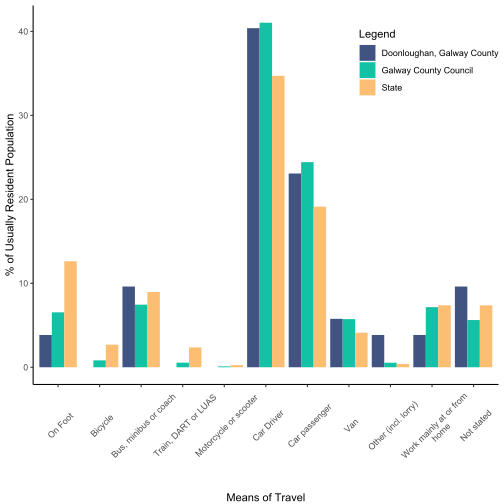
\includegraphics[width = 120mm]{../figures/TravelED.pdf}
	\caption{Percentage of Usually Resident Population by Means of Travel to Work, School, College or Childcare for a, Health Region and State; Census 2022.}
	\label{fig:vbnv}
	\end{figure}

\begin{table}[h]	
\centering
		\begin{tabular}{lTTTTTT}
  \hline
  \textbf{Means of travel} & \multicolumn{2}{c}{\textbf{a}} & \textbf{IHA}& \textbf{HSE Dublin and South East} & \textbf{State}\\ 
 \cline{2-3} \\
 & \emph{\textbf{Persons}} & \emph{\textbf{\%}} & \emph{\textbf{\%}} & \emph{\textbf{\%}} & \emph{\textbf{\%}} \\
 On Foot & \num{14} & 2.5 & 1.8& 12.7 & 12.6 \\
Bicycle & \num{1} & 0.2 & 0.0 & 3.1 & 2.7 \\
Bus, minibus or coach & \num{32} & 5.7 & 7.1 & 7.5 & 9.0 \\
Train, DART or LUAS & \num{7} & 1.2 & 0.9& 3.9 & 2.4 \\
Motorcycle or scooter & \num{0} & 0.0 & 0.0 & 0.3 & 0.3 \\
Car Driver & \num{243} & 43.1 &  41.7 & 34.4 & 34.7 \\
Car passenger & \num{153} & 27.1 & 26.5 & 19.6 & 19.1 \\
Van & \num{24} & 4.3 & 3.9& 3.7 & 4.1 \\
Other (incl. lorry) & \num{5} & 0.9 & 1.5& 0.4 & 0.4 \\
Work mainly at or from home & \num{57} & 10.1 & 9.5 & 8.6 & 7.4 \\
Not stated & \num{28} & 5.0 & 7.1 & 5.7 & 7.4 \\
Total & \num{564} & 100.0 & 100.0& 100.0 & 100.0 \\
  \hline
       \multicolumn{5}{l}{\href{https://data.cso.ie/table/SAP2022T11T1ED}{https://data.cso.ie/table/SAP2022T11T1ED}} &
\end{tabular}

\caption{Percentage of Usually Resident Population by Means of Travel to Work, School, College or Childcare for a; Census 2022. Percentage breakdowns for Health Region and State are also provided for comparison purposes.}
\end{table} 

\pagebreak

\section{Renewable Energy}\label{sect:RE}
\begin{figure}[H]
	\centering
	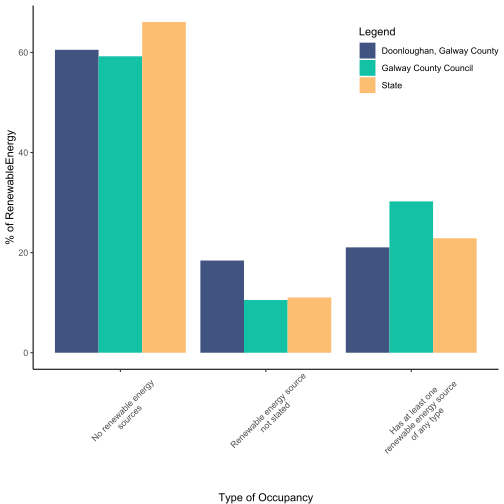
\includegraphics[width = 140mm]{../figures/RenewableEnergyED.pdf}
	\caption{Percentage of Households by Renewable Energy Source for a, Health Region and State; Census 2022.}
	\label{fig:vbnv}
	\end{figure}

\begin{table}[h]	
\centering
		\begin{tabular}{lTTTTT}
  \hline
  \textbf{Renewable Energy Source} & \multicolumn{2}{c}{\textbf{a}} & \textbf{IHA}& \textbf{HSE Dublin and South East} & \textbf{State}\\ 
 \cline{2-3} \\
 & \emph{\textbf{Households}} & \emph{\textbf{\%}} & \emph{\textbf{\%}} & \emph{\textbf{\%}}& \emph{\textbf{\%}} \\
 All households & \num{253} & 100.0 & 100.0 & 100.0 & 100.0 \\
  No renewable energy sources & \num{121} & 47.8 & 51.1& 64.8 & 66.1 \\
   Renewable energy source not stated & \num{19} & 7.5 & 8.9& 9.6 & 11.0 \\
    Has at least one renewable energy source of any type & \num{113} & 44.7 & 40.0& 25.7 & 22.9 \\
  \hline
       \multicolumn{5}{l}{\href{https://data.cso.ie/table/SAP2022T6T10ED}{https://data.cso.ie/table/SAP2022T6T10ED}} &
\end{tabular}

\caption{Percentage of Households by Renewable Energy Source for a; Census 2022. Percentage breakdowns for Health Region and State are also provided for comparison purposes.}
\end{table} 

\pagebreak

\section{Detailed Tables}\label{sect:ST}
\begin{table}[h]	
\centering
		\begin{tabular}{KTTTT}
  \hline
& \textbf{CHN} & \textbf{IHA} & \textbf{HR} & \textbf{State}\\ 
\hline
  \multicolumn{5}{l}{\textbf{Age (Percentage of population (excl. Dependency ratios))} }\\ 
\hline
Age Dependency Ratio & 55.9 & 55.2 & 53.2 \\
Youth Dependency Ratio & 30.8 & 29.7 & 30.1\\
Old Age Dependency Ratio & 25.1 & 17.8& 25.5 & 23.1\\ 
    \arrayrulecolor{lightgray}\hline
0-14 & 19.7 & 22.4& 19 & 19.6 \\ 
15-64 & 64.1 & 65.9& 64.7 & 65.4 \\ 
65+ & 16.2 & 11.6& 16.5 & 15 \\ 
  \arrayrulecolor{black}\hline
    \multicolumn{5}{l}{\textbf{Education (Percentage of those aged 15+)}}\\
    \arrayrulecolor{black}\hline
No formal education & 0.8& 1.1& 2.1& 2.4\\
Primary education & 8.6& 6.1& 6.7& 7.4\\
Lower secondary & 14.1& 14.1& 12.9& 13.2\\
Upper secondary & 14.5& 13.4& 17.4& 18.1\\
Technical or vocational qualification  & 7.6& 9.7& 7.2& 7.5\\
Advanced certificate/Completed apprenticeship & 8.8& 8.7& 5.5& 5.6\\
Higher certificate & 7.4& 6.1& 5.5& 5.5\\
Ordinary bachelor degree or national diploma & 7.6& 6.9& 8.2& 8.1\\
Hns bach. degree, prof. qual. or both & 16.2& 18.4& 14.6& 13.3\\
Postgraduate diploma or degree & 11.3& 10.5& 13.3& 11.2\\
Doctorate(Ph.D) or higher & 0.6& 0.4& 1.4& 1.1\\
  \arrayrulecolor{black}\hline
    \multicolumn{5}{l}{\textbf{Employment (Percentage of those aged 15+)}}\\ 
    \arrayrulecolor{black}\hline
At work & 58.4& 64.9& 55.1& 56.1\\
Looking for first regular job & 0.2& 0.0& 0.8& 0.8\\
short Term Unemployed  & 1.0& 0.0& 1.6& 1.7\\
Long Term Unemployed  & 2.0& 1.5& 2.5& 2.6\\
Student  & 11.3& 12.0& 11.0& 11.1\\
Looking after home/family   & 6.0& 6.2&& 6.9& 6.6\\
Retired  & 17.3& 11.7& 17.2& 15.9\\
Unable to work - perm. sickness or disability & 3.6& 3.7& 4.4& 4.6\\
\hline
    \multicolumn{5}{l}{\textbf{Employment (Percentage of those at work)}}\\
    \hline
Agriculture, forestry and fishing  & 11.2& 10.4&  4.0&  3.5\\
Building and construction & 5.3& 4.3& 5.4& 5.8\\
Manufacturing industries & 11.5& 14.2& 10.8& 11.8\\
Commerce and trade  & 16.8& 16.1& 26.4& 23.8\\
Transport and communications  & 8.1& 8.1& 9.5& 9.2\\
Public administration & 9.5& 9.5& 5.0& 5.7\\
Professional services & 27.4& 27.5& 24.3& 24.5\\
%Other & & 14.6& 15.8\\
\arrayrulecolor{black}\hline
    \multicolumn{5}{l}{\textbf{Social Class (Percentage of population)}}\\ 
    \arrayrulecolor{black}\hline
Professional workers  &  9.8& 11.011.1&  9.3\\
Managerial and technical & 37.6& 38.4& 33.2& 30.7\\
Non-manual & 16.0& 12.4& 15.7& 16.2\\
Skilled manual & 16.2& 16.9& 11.8& 12.9\\
Semi-skilled &  9.9&  9.5& 10.6& 11.2\\
Unskilled  & 2.4& 3.1& 2.8& 3.1\\
\end{tabular}
\end{table}
\pagebreak
\begin{table}[h]	
\centering
		\begin{tabular}{KTTTT}
  \arrayrulecolor{black}\hline
& \textbf{CHN} & \textbf{IHA} & \textbf{HR}& \textbf{State}\\ 
\hline
   \multicolumn{5}{l}{\textbf{Families (Percentage of family units)}}\\ 
   \arrayrulecolor{black}\hline
Families without children & 28.2& 25.4&32.1& 30.8\\
Families with 1 child & 24.4& 22.8&27.2& 27.1\\
Families with 2 children & 29.6& 31.625.0& 25.3\\
Families with 3 children & 13.6& 13.2&11.8& 12.3\\
Families with 4 children & 3.3& 5.3& 3.1& 3.5\\
Families with 5 or more children & 0.9& 1.8&0.8& 1.0\\
    \arrayrulecolor{lightgray}\hline
Couples with children & 61.5& 64.9&51.1& 52.0\\
Lone parent (mother) &  8.0&  7.0& 14.2& 14.6\\
Lone parent (father) & 2.3& 2.6& 2.6& 2.6\\
    \arrayrulecolor{lightgray}\hline
Pre-family families & 4.7& 5.3&9.0& 9.3\\
Empty nest families & 8.0& 8.8& 9.9& 9.4\\
Retired families & 15.5& 11.4&13.2& 12.0\\
Per-school families & 6.1& 8.8& 7.8& 8.1\\
Early school families & 8.0& 5.3&9.8& 9.9\\
Pre-adolescent families & 14.6& 19.3&11.6& 11.9\\
Adolescent families & 13.1& 14.9&12.1& 12.3\\
Adult families & 61.5& 26.3& 26.6& 27.0\\
    \arrayrulecolor{lightgray}\hline
Families with youngest child aged 0 - 4 & 17.6& 20.0&23.0& 14.6\\
Families with youngest child aged 5 - 9 & 17.6& 20.0&18.0& 18.1\\
Families with youngest child aged 10 - 14 & 17.6& 21.2&16.9& 16.9\\
Families with youngest child aged 15 - 19 & 16.3& 15.3&14.0& 13.6\\
Families with youngest child aged 20 and over & 30.7& 23.5&28.2& 27.5\\
\arrayrulecolor{black}\hline
    \multicolumn{5}{l}{\textbf{Health (Percentage of population)}}\\ 
    \arrayrulecolor{black}\hline
Very good general health & 57.9& 58.9&55.4& 53.2\\
Good general health & 30.1& 29.8& 29.3& 29.7\\
Fair general health & 7.9& 5.7&8.5& 8.6\\
Bad general health & 1.4& 1.2&1.4& 1.4\\
Very bad general health & 0.4& 0.5&0.3& 0.3\\
    \arrayrulecolor{lightgray}\hline
Persons who smoke &  8.2&  7.9&12.8& 13.1\\
    \arrayrulecolor{lightgray}\hline
With a disability (to some or to a great extent) & 22.0& 19.1&22.5& 21.5\\
\arrayrulecolor{black}\hline
    \multicolumn{5}{l}{\textbf{Household composition (Percentage of Private Households)}}\\ 
    \arrayrulecolor{black}\hline
Married couple households & 18.8& 16.8& 15.8& 14.9\\
Cohabiting couple households & 2.0& 2.2& 4.5& 4.3\\
Married couple with children households & 44.7& 47.4& 29.1& 29.4\\
Cohabiting couple with children households & 2.7& 3.6& 4.2& 4.3\\
One parent family (father) with  children households & 2.0& 2.2& 1.5& 1.5\\
One parent family (mother) and children households & 5.1& 4.4& 8.2& 8.5\\
Couple and others households  & 0.4& 0.7& 1.4& 1.5\\
Two or more non-related persons households & 2.0& 2.9& 4.7& 5.4\\
    \arrayrulecolor{lightgray}\hline
1 person households & 14.9& 15.3& 23.6& 23.1\\
2 person households & 25.5& 21.9& 29.9& 29.0\\
3 person households & 19.6& 20.4& 17.6& 17.9\\
4 person households & 22.7& 24.8& 16.6& 16.9\\
5 person households & 12.9&  8.6&  8.9\\
6 person households & 3.1& 2.8& 3.0\\
7 person households & 0.8& 1.5& 0.7& 0.8\\
8 or more person households & 0.4& 0.0& 0.3& 0.4\\
\arrayrulecolor{black}\hline
    \multicolumn{5}{l}{\textbf{Housing (Percentage of permanent dwellings)}}\\ 
    \arrayrulecolor{black}\hline
Occupied & 93.4& 90.6& 88.6& 87.4\\
Temporarily absent & 0.7& 0.7& 1.8& 1.6\\
Unoccupied holiday homes & 0.4& 0.7& 2.7& 3.2\\
Other vacant dwellings & 5.5& 8.1& 6.8& 7.7\\
\hline
\end{tabular}
\end{table}
\pagebreak
\begin{table}[h]	
\centering
		\begin{tabular}{KTTTT}
 \arrayrulecolor{black} \hline
& \textbf{CHN} & \textbf{IHA}& \textbf{HR} & \textbf{State}\\ 
\hline
    \multicolumn{5}{l}{\textbf{Housing (Percentage of permanent private households)}}\\ 
    \arrayrulecolor{black}   \hline
Owned with mortgage or loan & 40.7& 51.1& 28.0& 28.9\\
Owned outright & 49.4& 38.5& 38.9& 37.0\\
Rented from private landlord &  4.7&  4.4& 17.6& 18.0\\
Rented from Local Authority & 0.8& 0.7& 8.4& 8.3\\
Rented from voluntary/co-operative housing body & 0.0& 0.0& 1.6& 1.6\\
Occupied free of rent & 1.2& 0.7& 1.8& 1.7\\
    \arrayrulecolor{lightgray}\hline
1 room & 0.0& 0.0& 0.3& 0.5\\
2 rooms & 0.4& 0.0& 3.7& 3.9\\
3 rooms & 2.0& 2.2& 8.2& 8.0\\
4 rooms &  4.7&  4.4& 11.7& 11.0\\
5 rooms & 12.6& 17.8& 23.3& 23.8\\
6 rooms & 26.9& 26.7& 18.7& 19.9\\
7 rooms & 26.1& 29.6& 14.2& 14.0\\
8 or more rooms & 26.5& 17.8& 17.5& 15.8\\
    \arrayrulecolor{lightgray}\hline
No central heating & 0.8& 0.0& 1.3& 1.2\\
    \arrayrulecolor{lightgray}\hline
Public main water supply & 15.4&  9.6& 81.1& 80.1\\
Group scheme with public source water supply & 0.8& 0.7& 2.0& 4.3\\
Group scheme with private source water supply & 1.6& 1.5& 1.6& 3.4\\
Other private source water supply & 81.4& 87.4& 13.7&  9.9\\
No water supply & 0.8& 0.7& 0.1& 0.1\\
\arrayrulecolor{black}\hline
    \multicolumn{4}{l}{\textbf{Housing (Percentage of private households)}}\\ 
    \arrayrulecolor{black}\hline
House/Bungalow & 98.8& 98.5& 86.4& 86.7\\
Flat/Apartment &  0.4&  0.0& 13.3& 13.0\\
Bed-Sit & 0.0& 0.0& 0.1& 0.1\\
Caravan/Mobile home & 0.8& 1.5& 0.2& 0.2\\
    \arrayrulecolor{lightgray}\hline
Built Pre 1919 & 11.1& 11.9& 10.5&  8.4\\
Built 1919 - 1945 & 7.1& 5.9& 6.4& 6.2\\
Built  1946 - 1960 & 4.0& 5.2& 7.7& 7.2\\
Built  1961 - 1970 & 1.6& 0.7& 7.3& 6.7\\
Built  1971 - 1980 & 12.6&  9.6& 12.1& 12.2\\
Built  1981 - 1990 & 12.6&  9.6& 10.5& 10.1\\
Built  1991 - 2000 & 12.6& 10.4& 13.6& 14.5\\
Built  2001 - 2010 & 29.2& 36.3& 22.4& 24.5\\
Built  2011 - 2015 & 3.2& 3.7& 2.6& 2.7\\
Built  2016 or later & 4.3& 5.2& 5.0& 5.1\\
\arrayrulecolor{black}\hline
    \multicolumn{5}{l}{\textbf{Marital Status (Percentage of population)}}\\
    \arrayrulecolor{black}\hline
Single & 46.6& 48.9& 52.5& 53.9\\
Married (incl. same sex civil partnership) & 46.2& 44.4& 38.0& 37.1\\
Separated  & 2.0& 2.1& 2.4& 2.3\\
Divorced  & 1.6& 1.4& 2.8& 2.6\\
Widowed & 3.7& 3.1& 4.3& 4.1\\
\arrayrulecolor{black}\hline
    \multicolumn{4}{l}{\textbf{Migration and ethnicity (Percentage of population)}}\\ 
   \arrayrulecolor{black} \hline
Speak english not well & 0.1& 0.0& 1.3& 1.6\\
Speak english not at all & 0.3& 0.5& 0.2& 0.3\\
\arrayrulecolor{black}\hline
    \multicolumn{4}{l}{\textbf{Occupation (Percentage of those at work or unemployed)}}\\
   \arrayrulecolor{black} \hline
Managers, directors and senior officials &  9.8& 11.1&  9.0&  7.7\\
Professional occupations & 18.4& 17.1& 22.8& 20.3\\
Associate professional and technical occupations & 13.8& 15.3& 12.7& 11.7\\
Administrative and secretarial occupations & 7.7& 6.5& 8.6& 9.2\\
Skilled trades occupations & 21.5& 21.8& 12.4& 12.6\\
Caring, leisure and other service occupations & 7.2& 7.4& 7.0& 7.4\\
Sales and customer service occupations & 3.5& 1.4& 6.0& 6.2\\
Process, plant and machine operatives & 6.4& 6.0& 6.2& 6.9\\
Elementary occupations & 6.6& 7.9& 7.3& 8.2\\
\arrayrulecolor{black}\hline
\end{tabular}
\end{table}
\pagebreak
\begin{table}[h]	
\centering
		\begin{tabular}{KTTTT}
 \arrayrulecolor{black} \hline
& \textbf{CHN} & \textbf{IHA} & \textbf{HR}& \textbf{State}\\ 
 \arrayrulecolor{black} \hline
    \multicolumn{5}{l}{\textbf{Migration and ethnicity (Percentage of usually resident population)}}\\ 
    \arrayrulecolor{black}\hline
Ireland - Birthplace & 94.8& 95.2& 81.4& 80.0\\
UK - Birthplace & 2.0& 2.2& 5.6& 5.7\\
Poland - Birthplace & 0.3& 0.0& 1.8& 2.1\\
India - Birthplace & 0.4& 0.0& 1.2& 1.1\\
Other EU28 - Birthplace & 1.0& 0.7& 3.8& 4.4\\
Rest of world - Birthplace & 1.6& 1.9& 6.3& 6.7\\
    \arrayrulecolor{lightgray}\hline
White Irish & 92.7& 93.8& 79.6& 76.6\\
White Irish Traveller & 1.2& 0.0& 0.6& 0.6\\
Other White & 2.2& 1.2& 9.3& 9.9\\
Black or Black Irish & 0.0& 0.0& 0.8& 1.5\\
Asian or Asian Irish & 0.9& 0.5& 3.2& 3.3\\
Other ethnic or cultural background & 1.0& 1.4& 1.9& 2.0\\
    \arrayrulecolor{lightgray}\hline
Usual residence 1 year before census day - Outside Ireland & 0.3& 0.0& 1.9& 1.8\\

\arrayrulecolor{black}\hline
    \multicolumn{5}{l}{\textbf{Socio-economic group of ref. person (percentage of private households)}}\\ 
    \arrayrulecolor{black}\hline
A Employers and managers & 16.5& 16.8& 14.7& 12.9\\
B Higher professional & 0.8& 1.5& 2.1& 1.5\\
C Lower professional & 5.1& 5.8& 7.3& 6.3\\
D Non-manual & 28.6& 24.1& 34.0& 34.2\\
E Manual skilled & 11.0&  7.7&  8.5\\
F Semi-skilled & 6.3& 6.6& 6.9& 7.7\\
G Unskilled & 2.7& 3.6& 2.9& 3.2\\
H Own account workers & 5.1& 5.1& 3.8& 4.0\\
I Farmers & 11.8& 13.9&  3.0&  3.1\\
J Agricultural workers & 2.4& 0.7& 1.2& 1.2\\
Z All others gainfully occupied and unknown &  9.8& 10.2& 16.3& 17.5\\
\hline
\arrayrulecolor{black}\hline
    \multicolumn{5}{l}{\textbf{Transport (Percentage of population agCHN 5+)}}\\ 
   \arrayrulecolor{black} \hline
No motor car (percentage of households) &  3.6&  3.0& 12.7& 
13.4\\
    \arrayrulecolor{lightgray}\hline
\emph{Travel to work, school, College or childcare:} & & & \\
\quad On Foot &  2.5&  1.8& 12.7& 12.6\\
\quad By Bicycle & 0.2& 0.0& 3.1& 2.7\\
\quad By Bus, minibus or coach & 5.7& 7.1& 7.5& 9.0\\
\quad By Train, DART or LUAS & 1.2& 0.9& 3.9& 2.4\\
\quad By Motorcycle or scooter & 0.0& 0.0& 0.3& 0.3\\
\quad Car driver & 43.1& 34.4& 34.7\\
\quad Car passenger & 27.1& 26.5& 19.6& 19.1\\
\quad By Van & 4.3& 3.9& 3.7& 4.1\\
\quad By Other (incl. lorry) & 0.9& 1.5& 0.4& 0.4\\
    \arrayrulecolor{lightgray}\hline
Work mainly at or from home & 10.1&  9.5&  8.6&  7.4\\
Journey time to work, school or college is Under 15 mins & 38.1& 38.1& 30.6& 29.4\\
Journey time to work, school or college is 1/4 hour - under 1/2 hour & 26.9& 28.2& 29.2& 28.1\\
Journey time to work, school or college is 1/2 hour - under 3/4 hour & 12.2&  9.3& 17.1& 17.3\\
Journey time to work, school or college is 3/4 hour - under 1 hour & 4.8& 6.5& 5.8& 5.9\\
Journey time to work, school or college is 1 hour - under 1 1/2 hours & 6.6& 6.9& 5.9& 6.1\\
Journey time to work, school or college is 1 1/2 hours and over & 4.1& 3.4& 2.7& 2.5\\
\arrayrulecolor{black}\hline
    \multicolumn{5}{l}{\textbf{Other}}\\ 
    \arrayrulecolor{black}\hline
Has renewable energy source (percentage of permanent private households) & 44.7& 40.0& 25.7& 22.9\\
    \arrayrulecolor{lightgray}\hline
Volunteers (percentage of population) & 16.1& 12.6& 14.2& 13.8\\
    \arrayrulecolor{lightgray}\hline
No internet connection& 9.5& 6.7& 8.3& 8.7\\
\arrayrulecolor{black}\hline
\end{tabular}
\end{table}


\end{document}
